% Options for packages loaded elsewhere
\PassOptionsToPackage{unicode}{hyperref}
\PassOptionsToPackage{hyphens}{url}
%
\documentclass[
]{article}
\usepackage{amsmath,amssymb}
\usepackage{iftex}
\ifPDFTeX
  \usepackage[T1]{fontenc}
  \usepackage[utf8]{inputenc}
  \usepackage{textcomp} % provide euro and other symbols
\else % if luatex or xetex
  \usepackage{unicode-math} % this also loads fontspec
  \defaultfontfeatures{Scale=MatchLowercase}
  \defaultfontfeatures[\rmfamily]{Ligatures=TeX,Scale=1}
\fi
\usepackage{lmodern}
\ifPDFTeX\else
  % xetex/luatex font selection
\fi
% Use upquote if available, for straight quotes in verbatim environments
\IfFileExists{upquote.sty}{\usepackage{upquote}}{}
\IfFileExists{microtype.sty}{% use microtype if available
  \usepackage[]{microtype}
  \UseMicrotypeSet[protrusion]{basicmath} % disable protrusion for tt fonts
}{}
\makeatletter
\@ifundefined{KOMAClassName}{% if non-KOMA class
  \IfFileExists{parskip.sty}{%
    \usepackage{parskip}
  }{% else
    \setlength{\parindent}{0pt}
    \setlength{\parskip}{6pt plus 2pt minus 1pt}}
}{% if KOMA class
  \KOMAoptions{parskip=half}}
\makeatother
\usepackage{xcolor}
\usepackage[margin=1in]{geometry}
\usepackage{longtable,booktabs,array}
\usepackage{calc} % for calculating minipage widths
% Correct order of tables after \paragraph or \subparagraph
\usepackage{etoolbox}
\makeatletter
\patchcmd\longtable{\par}{\if@noskipsec\mbox{}\fi\par}{}{}
\makeatother
% Allow footnotes in longtable head/foot
\IfFileExists{footnotehyper.sty}{\usepackage{footnotehyper}}{\usepackage{footnote}}
\makesavenoteenv{longtable}
\usepackage{graphicx}
\makeatletter
\def\maxwidth{\ifdim\Gin@nat@width>\linewidth\linewidth\else\Gin@nat@width\fi}
\def\maxheight{\ifdim\Gin@nat@height>\textheight\textheight\else\Gin@nat@height\fi}
\makeatother
% Scale images if necessary, so that they will not overflow the page
% margins by default, and it is still possible to overwrite the defaults
% using explicit options in \includegraphics[width, height, ...]{}
\setkeys{Gin}{width=\maxwidth,height=\maxheight,keepaspectratio}
% Set default figure placement to htbp
\makeatletter
\def\fps@figure{htbp}
\makeatother
\setlength{\emergencystretch}{3em} % prevent overfull lines
\providecommand{\tightlist}{%
  \setlength{\itemsep}{0pt}\setlength{\parskip}{0pt}}
\setcounter{secnumdepth}{-\maxdimen} % remove section numbering
\ifLuaTeX
  \usepackage{selnolig}  % disable illegal ligatures
\fi
\IfFileExists{bookmark.sty}{\usepackage{bookmark}}{\usepackage{hyperref}}
\IfFileExists{xurl.sty}{\usepackage{xurl}}{} % add URL line breaks if available
\urlstyle{same}
\hypersetup{
  pdftitle={Data Analysis Climate Law Study},
  pdfauthor={Nina Frings \& Julius Fenn},
  hidelinks,
  pdfcreator={LaTeX via pandoc}}

\title{Data Analysis Climate Law Study}
\author{Nina Frings \& Julius Fenn}
\date{2023-09-06}

\begin{document}
\maketitle

{
\setcounter{tocdepth}{3}
\tableofcontents
}
\hypertarget{analysis}{%
\subsection{Analysis}\label{analysis}}

\hypertarget{descriptive-statistics-sample}{%
\subsubsection{Descriptive statistics
sample}\label{descriptive-statistics-sample}}

\textbf{Participants in first wave: 351}\\
\textbf{Participants that completed both wavves: 254}\\
\textbf{Additional ``control group'' partcipants: 72}

\textbf{percentage of overall sample that completed wave 1 and wave 2}

\begin{longtable}[]{@{}lllll@{}}
\toprule\noalign{}
& divers & Keine Angabe & männlich & weiblich \\
\midrule\noalign{}
\endhead
\bottomrule\noalign{}
\endlastfoot
18-29 & 0 & 0 & 14 & 8 \\
30-39 & 0 & 0 & 12 & 10 \\
40-49 & 0 & 0 & 10 & 7 \\
50-59 & 0 & 0 & 11 & 13 \\
60-80 & 0 & 0 & 11 & 4 \\
\end{longtable}

\textbf{Political party identification}

\begin{center}\includegraphics{02_analysis_files/figure-latex/unnamed-chunk-4-1} \end{center}

\hypertarget{media-climate-change-concern}{%
\paragraph{Media, climate change
concern}\label{media-climate-change-concern}}

\hypertarget{climate-change-concern}{%
\paragraph{Climate change concern}\label{climate-change-concern}}

Cronbachs's alpha of 0.95, skew of -0.99

\begin{center}\includegraphics{02_analysis_files/figure-latex/unnamed-chunk-5-1} \end{center}

By party

\begin{center}\includegraphics{02_analysis_files/figure-latex/unnamed-chunk-7-1} \end{center}

\hypertarget{media-engagement}{%
\paragraph{Media engagement}\label{media-engagement}}

The items were phrased as: How did you inform yourself about the climate
law and the vote \textbf{in the past month}

Cronbachs alpha of 0.89

Type of media used as information source

\begin{center}\includegraphics{02_analysis_files/figure-latex/unnamed-chunk-10-1} \end{center}

\hypertarget{news-media}{%
\paragraph{News media}\label{news-media}}

Newspapers used as source of information

\begin{center}\includegraphics{02_analysis_files/figure-latex/unnamed-chunk-13-1} \end{center}

\begin{center}\includegraphics{02_analysis_files/figure-latex/unnamed-chunk-14-1} \end{center}

\hypertarget{correlations-between-predictor-variables-cc-concern-rating-of-law-and-political-orientation}{%
\subsubsection{Correlations between predictor variables cc concern,
rating of law and political
orientation:}\label{correlations-between-predictor-variables-cc-concern-rating-of-law-and-political-orientation}}

\begin{center}\includegraphics{02_analysis_files/figure-latex/unnamed-chunk-15-1} \end{center}

\hypertarget{cam-indicators}{%
\subsubsection{CAM Indicators}\label{cam-indicators}}

\begin{center}\includegraphics{02_analysis_files/figure-latex/unnamed-chunk-16-1} \end{center}

\begin{center}\includegraphics{02_analysis_files/figure-latex/unnamed-chunk-16-2} \end{center}

Did people change the valence of ``Klimagesetz''?

\begin{longtable}[]{@{}lrrr@{}}
\toprule\noalign{}
& t1 & t2 & wave2\_control \\
\midrule\noalign{}
\endhead
\bottomrule\noalign{}
\endlastfoot
-3 & 11 & 3 & 2 \\
-2 & 2 & 5 & 1 \\
-1 & 4 & 2 & 0 \\
0 & 207 & 223 & 60 \\
1 & 8 & 8 & 2 \\
2 & 14 & 6 & 3 \\
3 & 7 & 6 & 4 \\
\end{longtable}

\textbf{Macro indicators}

\begin{verbatim}
## `stat_bin()` using `bins = 30`. Pick better value with `binwidth`.
\end{verbatim}

\begin{center}\includegraphics{02_analysis_files/figure-latex/unnamed-chunk-19-1} \end{center}

\begin{verbatim}
##                                          Mean   SD Median CoeffofVariation
## mean_valence_macro_t1                    0.11 0.94   0.11             8.61
## mean_valence_normed_macro_t1             0.06 0.38   0.00             6.60
## density_macro_t1                         0.27 0.09   0.25             0.33
## transitivity_macro_t1                    0.14 0.18   0.00             1.26
## centr_degree_macro_t1                    0.47 0.23   0.42             0.50
## centr_clo_macro_t1                       0.61 0.23   0.56             0.38
## centr_betw_macro_t1                      0.66 0.23   0.67             0.35
## centr_eigen_macro_t1                     0.63 0.10   0.65             0.16
## meanDistance_directed_macro_t1           2.11 0.41   2.06             0.20
## meanDistance_undirected_macro_t1         2.11 0.41   2.06             0.20
## diameter_weighted_undirected_macro_t1    3.54 1.23   4.00             0.35
## diameter_unweighted_undirected_macro_t1  3.54 1.23   4.00             0.35
## diameter_unweighted_directed_macro_t1    3.54 1.23   4.00             0.35
## num_nodes_macro_t1                       9.63 2.18   9.00             0.23
## num_nodes_pos_macro_t1                   3.75 2.35   4.00             0.63
## num_nodes_neg_macro_t1                   3.21 2.38   3.00             0.74
## num_nodes_neut_macro_t1                  1.67 1.75   1.00             1.04
## num_nodes_ambi_macro_t1                  1.00 1.31   1.00             1.31
## num_edges_macro_t1                      21.46 7.37  20.00             0.34
## num_edges_solid_macro_t1                21.46 7.37  20.00             0.34
## num_edges_dashed_macro_t1                0.00 0.00   0.00              NaN
## num_edges_invaliddashed_macro_t1         1.08 1.65   0.00             1.53
## meanWeightEdges_macro_t1                 1.00 0.00   1.00             0.00
## reciprocity_macro_t1                     1.00 0.00   1.00             0.00
## assortativity_valence_macro_t1          -0.21 0.30  -0.20            -1.46
## assortativityDegree_macro_t1            -0.52 0.28  -0.51            -0.54
##                                         Minimum Maximun Lower Quantile
## mean_valence_macro_t1                     -3.00    2.88          -3.00
## mean_valence_normed_macro_t1              -1.00    1.00          -1.00
## density_macro_t1                           0.08    0.64           0.08
## transitivity_macro_t1                      0.00    0.69           0.00
## centr_degree_macro_t1                      0.00    0.89           0.00
## centr_clo_macro_t1                         0.00    1.00           0.00
## centr_betw_macro_t1                        0.00    1.00           0.00
## centr_eigen_macro_t1                       0.00    0.79           0.00
## meanDistance_directed_macro_t1             1.36    3.67           1.36
## meanDistance_undirected_macro_t1           1.36    3.67           1.36
## diameter_weighted_undirected_macro_t1      2.00    8.00           2.00
## diameter_unweighted_undirected_macro_t1    2.00    8.00           2.00
## diameter_unweighted_directed_macro_t1      2.00    8.00           2.00
## num_nodes_macro_t1                         8.00   27.00           8.00
## num_nodes_pos_macro_t1                     0.00   22.00           0.00
## num_nodes_neg_macro_t1                     0.00   17.00           0.00
## num_nodes_neut_macro_t1                    0.00   10.00           0.00
## num_nodes_ambi_macro_t1                    0.00    8.00           0.00
## num_edges_macro_t1                        14.00   56.00          14.00
## num_edges_solid_macro_t1                  14.00   56.00          14.00
## num_edges_dashed_macro_t1                  0.00    0.00           0.00
## num_edges_invaliddashed_macro_t1           0.00    9.00           0.00
## meanWeightEdges_macro_t1                   1.00    1.00           1.00
## reciprocity_macro_t1                       1.00    1.00           1.00
## assortativity_valence_macro_t1            -1.00    0.59          -1.00
## assortativityDegree_macro_t1              -1.00    0.13          -1.00
##                                         Upper Quantile Skewness Kurtosis(-3)
## mean_valence_macro_t1                             2.88    -0.63         1.67
## mean_valence_normed_macro_t1                      1.00    -0.33         0.53
## density_macro_t1                                  0.64     1.37         2.49
## transitivity_macro_t1                             0.69     0.98        -0.22
## centr_degree_macro_t1                             0.89     0.33        -1.08
## centr_clo_macro_t1                                1.00     0.23        -1.00
## centr_betw_macro_t1                               1.00    -0.37        -0.46
## centr_eigen_macro_t1                              0.79    -1.52         4.74
## meanDistance_directed_macro_t1                    3.67     0.87         0.81
## meanDistance_undirected_macro_t1                  3.67     0.87         0.81
## diameter_weighted_undirected_macro_t1             8.00     0.58         0.09
## diameter_unweighted_undirected_macro_t1           8.00     0.58         0.09
## diameter_unweighted_directed_macro_t1             8.00     0.58         0.09
## num_nodes_macro_t1                               27.00     3.88        21.49
## num_nodes_pos_macro_t1                           22.00     2.15        14.10
## num_nodes_neg_macro_t1                           17.00     1.53         5.06
## num_nodes_neut_macro_t1                          10.00     2.28         6.17
## num_nodes_ambi_macro_t1                           8.00     2.42         8.78
## num_edges_macro_t1                               56.00     1.94         4.75
## num_edges_solid_macro_t1                         56.00     1.94         4.75
## num_edges_dashed_macro_t1                         0.00      NaN          NaN
## num_edges_invaliddashed_macro_t1                  9.00     1.94         3.85
## meanWeightEdges_macro_t1                          1.00      NaN          NaN
## reciprocity_macro_t1                              1.00      NaN          NaN
## assortativity_valence_macro_t1                    0.59    -0.06        -0.15
## assortativityDegree_macro_t1                      0.13    -0.01        -0.69
##                                         KS-Test
## mean_valence_macro_t1                      0.01
## mean_valence_normed_macro_t1               0.00
## density_macro_t1                           0.00
## transitivity_macro_t1                      0.00
## centr_degree_macro_t1                      0.01
## centr_clo_macro_t1                         0.00
## centr_betw_macro_t1                        0.17
## centr_eigen_macro_t1                       0.01
## meanDistance_directed_macro_t1             0.02
## meanDistance_undirected_macro_t1           0.02
## diameter_weighted_undirected_macro_t1      0.00
## diameter_unweighted_undirected_macro_t1    0.00
## diameter_unweighted_directed_macro_t1      0.00
## num_nodes_macro_t1                         0.00
## num_nodes_pos_macro_t1                     0.00
## num_nodes_neg_macro_t1                     0.00
## num_nodes_neut_macro_t1                    0.00
## num_nodes_ambi_macro_t1                    0.00
## num_edges_macro_t1                         0.00
## num_edges_solid_macro_t1                   0.00
## num_edges_dashed_macro_t1                  0.00
## num_edges_invaliddashed_macro_t1           0.00
## meanWeightEdges_macro_t1                   0.00
## reciprocity_macro_t1                       0.00
## assortativity_valence_macro_t1             0.98
## assortativityDegree_macro_t1               0.21
\end{verbatim}

\textbf{Micro indicators}

\begin{verbatim}
## `stat_bin()` using `bins = 30`. Pick better value with `binwidth`.
\end{verbatim}

\begin{center}\includegraphics{02_analysis_files/figure-latex/unnamed-chunk-20-1} \end{center}

\begin{verbatim}
##                                 Mean   SD Median CoeffofVariation Minimum
## degreetot_micro_Klimagesetz_t1 10.45 4.16     10             0.40     2.0
## valence_micro_Klimagesetz_t1    0.06 0.97      0            17.32    -3.0
## centr_clo_micro_Klimagesetz_t1  0.96 0.10      1             0.10     0.5
##                                Maximun Lower Quantile Upper Quantile Skewness
## degreetot_micro_Klimagesetz_t1      22            2.0             22     0.10
## valence_micro_Klimagesetz_t1         3           -3.0              3    -0.24
## centr_clo_micro_Klimagesetz_t1       1            0.5              1    -2.88
##                                Kurtosis(-3) KS-Test
## degreetot_micro_Klimagesetz_t1        -0.81       0
## valence_micro_Klimagesetz_t1           4.93       0
## centr_clo_micro_Klimagesetz_t1         8.04       0
\end{verbatim}

\hypertarget{for-difference-values}{%
\subparagraph{For difference values}\label{for-difference-values}}

\textbf{Macro indicators}

\begin{verbatim}
## `stat_bin()` using `bins = 30`. Pick better value with `binwidth`.
\end{verbatim}

\begin{center}\includegraphics{02_analysis_files/figure-latex/unnamed-chunk-23-1} \end{center}

\begin{verbatim}
##                                          Mean   SD Median CoeffofVariation
## mean_valence_macro_t1                    0.00 0.80   0.00          -267.78
## mean_valence_normed_macro_t1             0.00 0.35   0.00            85.89
## density_macro_t1                        -0.01 0.11   0.00           -12.57
## transitivity_macro_t1                   -0.01 0.21   0.00           -19.07
## centr_degree_macro_t1                   -0.01 0.26   0.00           -21.79
## centr_clo_macro_t1                      -0.01 0.27   0.00           -48.97
## centr_betw_macro_t1                      0.00 0.28   0.00           363.15
## centr_eigen_macro_t1                     0.01 0.15   0.00            10.01
## meanDistance_directed_macro_t1          -0.01 0.51   0.00           -36.60
## meanDistance_undirected_macro_t1        -0.01 0.51   0.00           -36.60
## diameter_weighted_undirected_macro_t1   -0.03 1.59   0.00           -51.00
## diameter_unweighted_undirected_macro_t1  0.04 1.45   0.00            33.76
## diameter_unweighted_directed_macro_t1    0.04 1.45   0.00            33.76
## num_nodes_macro_t1                      -0.08 2.53   0.00           -32.35
## num_nodes_pos_macro_t1                   0.04 2.57   0.00            59.71
## num_nodes_neg_macro_t1                   0.12 2.20   0.00            18.18
## num_nodes_neut_macro_t1                 -0.48 1.91   0.00            -3.97
## num_nodes_ambi_macro_t1                  0.24 1.47   0.00             6.18
## num_edges_macro_t1                      -0.73 8.04   0.00           -11.07
## num_edges_solid_macro_t1                -0.73 8.04   0.00           -11.07
## num_edges_dashed_macro_t1                0.00 0.00   0.00              NaN
## num_edges_invaliddashed_macro_t1         0.04 1.91   0.00            44.46
## meanWeightEdges_macro_t1                -0.02 0.10   0.00            -5.57
## reciprocity_macro_t1                     0.00 0.00   0.00              NaN
## assortativity_valence_macro_t1           0.03 0.38   0.06            11.03
## assortativityDegree_macro_t1             0.04 0.32   0.01             7.22
## mean_valence_macro_t2                    0.12 1.01   0.09             8.72
## mean_valence_normed_macro_t2             0.05 0.37   0.00             6.90
## density_macro_t2                         0.28 0.11   0.25             0.41
## transitivity_macro_t2                    0.15 0.20   0.00             1.28
## centr_degree_macro_t2                    0.48 0.26   0.45             0.53
## centr_clo_macro_t2                       0.62 0.26   0.59             0.42
## centr_betw_macro_t2                      0.66 0.26   0.68             0.39
## centr_eigen_macro_t2                     0.62 0.13   0.65             0.22
## meanDistance_directed_macro_t2           2.12 0.53   1.96             0.25
## meanDistance_undirected_macro_t2         2.12 0.53   1.96             0.25
## diameter_weighted_undirected_macro_t2    3.58 1.51   3.00             0.42
## diameter_unweighted_undirected_macro_t2  3.50 1.38   3.00             0.39
## diameter_unweighted_directed_macro_t2    3.50 1.38   3.00             0.39
## num_nodes_macro_t2                       9.70 2.49   9.00             0.26
## num_nodes_pos_macro_t2                   3.70 2.52   4.00             0.68
## num_nodes_neg_macro_t2                   3.08 2.12   3.00             0.69
## num_nodes_neut_macro_t2                  2.16 2.28   1.00             1.06
## num_nodes_ambi_macro_t2                  0.77 1.17   0.00             1.53
## num_edges_macro_t2                      22.16 8.30  20.00             0.37
## num_edges_solid_macro_t2                22.16 8.30  20.00             0.37
## num_edges_dashed_macro_t2                0.00 0.00   0.00              NaN
## num_edges_invaliddashed_macro_t2         1.03 1.80   0.00             1.74
## meanWeightEdges_macro_t2                 1.02 0.10   1.00             0.09
## reciprocity_macro_t2                     1.00 0.00   1.00             0.00
## assortativity_valence_macro_t2          -0.24 0.31  -0.22            -1.31
## assortativityDegree_macro_t2            -0.56 0.29  -0.56            -0.51
##                                         Minimum Maximun Lower Quantile
## mean_valence_macro_t1                     -3.36    3.07          -3.36
## mean_valence_normed_macro_t1              -1.77    1.14          -1.77
## density_macro_t1                          -0.76    0.31          -0.76
## transitivity_macro_t1                     -0.96    0.60          -0.96
## centr_degree_macro_t1                     -0.88    0.73          -0.88
## centr_clo_macro_t1                        -1.00    0.78          -1.00
## centr_betw_macro_t1                       -1.00    0.80          -1.00
## centr_eigen_macro_t1                      -0.74    0.60          -0.74
## meanDistance_directed_macro_t1            -3.08    1.51          -3.08
## meanDistance_undirected_macro_t1          -3.08    1.51          -3.08
## diameter_weighted_undirected_macro_t1     -8.00    5.00          -8.00
## diameter_unweighted_undirected_macro_t1   -5.00    5.00          -5.00
## diameter_unweighted_directed_macro_t1     -5.00    5.00          -5.00
## num_nodes_macro_t1                       -15.00   10.00         -15.00
## num_nodes_pos_macro_t1                   -12.00   10.00         -12.00
## num_nodes_neg_macro_t1                    -6.00   17.00          -6.00
## num_nodes_neut_macro_t1                  -11.00    5.00         -11.00
## num_nodes_ambi_macro_t1                   -7.00    8.00          -7.00
## num_edges_macro_t1                       -32.00   24.00         -32.00
## num_edges_solid_macro_t1                 -32.00   24.00         -32.00
## num_edges_dashed_macro_t1                  0.00    0.00           0.00
## num_edges_invaliddashed_macro_t1          -7.00    7.00          -7.00
## meanWeightEdges_macro_t1                  -1.00    0.00          -1.00
## reciprocity_macro_t1                       0.00    0.00           0.00
## assortativity_valence_macro_t1            -1.00    0.97          -1.00
## assortativityDegree_macro_t1              -1.12    1.02          -1.12
## mean_valence_macro_t2                     -2.73    3.00          -2.73
## mean_valence_normed_macro_t2              -0.91    1.00          -0.91
## density_macro_t2                           0.08    0.96           0.08
## transitivity_macro_t2                      0.00    0.96           0.00
## centr_degree_macro_t2                      0.03    0.89           0.03
## centr_clo_macro_t2                         0.04    1.00           0.04
## centr_betw_macro_t2                        0.00    1.00           0.00
## centr_eigen_macro_t2                       0.04    0.81           0.04
## meanDistance_directed_macro_t2             1.04    4.83           1.04
## meanDistance_undirected_macro_t2           1.04    4.83           1.04
## diameter_weighted_undirected_macro_t2      2.00   10.00           2.00
## diameter_unweighted_undirected_macro_t2    2.00   10.00           2.00
## diameter_unweighted_directed_macro_t2      2.00   10.00           2.00
## num_nodes_macro_t2                         8.00   27.00           8.00
## num_nodes_pos_macro_t2                     0.00   18.00           0.00
## num_nodes_neg_macro_t2                     0.00   10.00           0.00
## num_nodes_neut_macro_t2                    0.00   14.00           0.00
## num_nodes_ambi_macro_t2                    0.00    7.00           0.00
## num_edges_macro_t2                        14.00   56.00          14.00
## num_edges_solid_macro_t2                  14.00   56.00          14.00
## num_edges_dashed_macro_t2                  0.00    0.00           0.00
## num_edges_invaliddashed_macro_t2           0.00   10.00           0.00
## meanWeightEdges_macro_t2                   1.00    2.00           1.00
## reciprocity_macro_t2                       1.00    1.00           1.00
## assortativity_valence_macro_t2            -1.00    0.71          -1.00
## assortativityDegree_macro_t2              -1.00    0.41          -1.00
##                                         Upper Quantile Skewness Kurtosis(-3)
## mean_valence_macro_t1                             3.07    -0.29         2.10
## mean_valence_normed_macro_t1                      1.14    -0.42         2.48
## density_macro_t1                                  0.31    -1.74         8.76
## transitivity_macro_t1                             0.60    -0.64         2.29
## centr_degree_macro_t1                             0.73    -0.35         0.80
## centr_clo_macro_t1                                0.78    -0.32         0.93
## centr_betw_macro_t1                               0.80    -0.13         0.88
## centr_eigen_macro_t1                              0.60     0.19         3.43
## meanDistance_directed_macro_t1                    1.51    -1.26         7.38
## meanDistance_undirected_macro_t1                  1.51    -1.26         7.38
## diameter_weighted_undirected_macro_t1             5.00    -0.71         3.28
## diameter_unweighted_undirected_macro_t1           5.00    -0.07         1.20
## diameter_unweighted_directed_macro_t1             5.00    -0.07         1.20
## num_nodes_macro_t1                               10.00    -1.04        10.01
## num_nodes_pos_macro_t1                           10.00    -0.09         3.58
## num_nodes_neg_macro_t1                           17.00     2.02        13.56
## num_nodes_neut_macro_t1                           5.00    -1.48         5.69
## num_nodes_ambi_macro_t1                           8.00     0.64         7.80
## num_edges_macro_t1                               24.00    -0.78         3.12
## num_edges_solid_macro_t1                         24.00    -0.78         3.12
## num_edges_dashed_macro_t1                         0.00      NaN          NaN
## num_edges_invaliddashed_macro_t1                  7.00    -0.01         3.80
## meanWeightEdges_macro_t1                          0.00    -7.20        58.10
## reciprocity_macro_t1                              0.00      NaN          NaN
## assortativity_valence_macro_t1                    0.97    -0.14        -0.24
## assortativityDegree_macro_t1                      1.02    -0.15         1.30
## mean_valence_macro_t2                             3.00    -0.41         1.24
## mean_valence_normed_macro_t2                      1.00    -0.27         0.69
## density_macro_t2                                  0.96     2.14         7.29
## transitivity_macro_t2                             0.96     1.18         0.80
## centr_degree_macro_t2                             0.89     0.22        -1.29
## centr_clo_macro_t2                                1.00     0.10        -1.14
## centr_betw_macro_t2                               1.00    -0.44        -0.62
## centr_eigen_macro_t2                              0.81    -1.38         1.75
## meanDistance_directed_macro_t2                    4.83     1.44         3.31
## meanDistance_undirected_macro_t2                  4.83     1.44         3.31
## diameter_weighted_undirected_macro_t2            10.00     1.20         1.97
## diameter_unweighted_undirected_macro_t2          10.00     0.97         1.40
## diameter_unweighted_directed_macro_t2            10.00     0.97         1.40
## num_nodes_macro_t2                               27.00     3.90        19.62
## num_nodes_pos_macro_t2                           18.00     1.24         4.36
## num_nodes_neg_macro_t2                           10.00     0.67         0.27
## num_nodes_neut_macro_t2                          14.00     2.33         5.70
## num_nodes_ambi_macro_t2                           7.00     2.13         5.65
## num_edges_macro_t2                               56.00     1.69         3.12
## num_edges_solid_macro_t2                         56.00     1.69         3.12
## num_edges_dashed_macro_t2                         0.00      NaN          NaN
## num_edges_invaliddashed_macro_t2                 10.00     2.34         5.87
## meanWeightEdges_macro_t2                          2.00     7.20        58.10
## reciprocity_macro_t2                              1.00      NaN          NaN
## assortativity_valence_macro_t2                    0.71     0.00        -0.24
## assortativityDegree_macro_t2                      0.41     0.22        -0.33
##                                         KS-Test
## mean_valence_macro_t1                      0.16
## mean_valence_normed_macro_t1               0.11
## density_macro_t1                           0.00
## transitivity_macro_t1                      0.00
## centr_degree_macro_t1                      0.00
## centr_clo_macro_t1                         0.01
## centr_betw_macro_t1                        0.14
## centr_eigen_macro_t1                       0.04
## meanDistance_directed_macro_t1             0.05
## meanDistance_undirected_macro_t1           0.05
## diameter_weighted_undirected_macro_t1      0.00
## diameter_unweighted_undirected_macro_t1    0.00
## diameter_unweighted_directed_macro_t1      0.00
## num_nodes_macro_t1                         0.00
## num_nodes_pos_macro_t1                     0.00
## num_nodes_neg_macro_t1                     0.00
## num_nodes_neut_macro_t1                    0.00
## num_nodes_ambi_macro_t1                    0.00
## num_edges_macro_t1                         0.00
## num_edges_solid_macro_t1                   0.00
## num_edges_dashed_macro_t1                  0.00
## num_edges_invaliddashed_macro_t1           0.00
## meanWeightEdges_macro_t1                   0.00
## reciprocity_macro_t1                       0.00
## assortativity_valence_macro_t1             0.94
## assortativityDegree_macro_t1               0.35
## mean_valence_macro_t2                      0.01
## mean_valence_normed_macro_t2               0.00
## density_macro_t2                           0.00
## transitivity_macro_t2                      0.00
## centr_degree_macro_t2                      0.01
## centr_clo_macro_t2                         0.01
## centr_betw_macro_t2                        0.03
## centr_eigen_macro_t2                       0.00
## meanDistance_directed_macro_t2             0.00
## meanDistance_undirected_macro_t2           0.00
## diameter_weighted_undirected_macro_t2      0.00
## diameter_unweighted_undirected_macro_t2    0.00
## diameter_unweighted_directed_macro_t2      0.00
## num_nodes_macro_t2                         0.00
## num_nodes_pos_macro_t2                     0.00
## num_nodes_neg_macro_t2                     0.00
## num_nodes_neut_macro_t2                    0.00
## num_nodes_ambi_macro_t2                    0.00
## num_edges_macro_t2                         0.00
## num_edges_solid_macro_t2                   0.00
## num_edges_dashed_macro_t2                  0.00
## num_edges_invaliddashed_macro_t2           0.00
## meanWeightEdges_macro_t2                   0.00
## reciprocity_macro_t2                       0.00
## assortativity_valence_macro_t2             0.84
## assortativityDegree_macro_t2               0.03
\end{verbatim}

\textbf{Micro indicators}

\begin{verbatim}
## `stat_bin()` using `bins = 30`. Pick better value with `binwidth`.
\end{verbatim}

\begin{center}\includegraphics{02_analysis_files/figure-latex/unnamed-chunk-24-1} \end{center}

\begin{verbatim}
##                                 Mean   SD Median CoeffofVariation Minimum
## degreetot_micro_Klimagesetz_t1 -0.66 4.79      0            -7.21  -20.00
## valence_micro_Klimagesetz_t1    0.00 1.00      0           248.99   -6.00
## centr_clo_micro_Klimagesetz_t1  0.00 0.12      0           -25.48   -0.50
## degreetot_micro_Klimagesetz_t2 11.13 4.35     12             0.39    2.00
## valence_micro_Klimagesetz_t2    0.07 0.73      0            10.85   -3.00
## centr_clo_micro_Klimagesetz_t2  0.97 0.09      1             0.09    0.48
##                                Maximun Lower Quantile Upper Quantile Skewness
## degreetot_micro_Klimagesetz_t1   14.00         -20.00          14.00    -0.35
## valence_micro_Klimagesetz_t1      3.00          -6.00           3.00    -0.81
## centr_clo_micro_Klimagesetz_t1    0.52          -0.50           0.52    -0.12
## degreetot_micro_Klimagesetz_t2   24.00           2.00          24.00    -0.15
## valence_micro_Klimagesetz_t2      3.00          -3.00           3.00     0.70
## centr_clo_micro_Klimagesetz_t2    1.00           0.48           1.00    -3.35
##                                Kurtosis(-3) KS-Test
## degreetot_micro_Klimagesetz_t1         0.93       0
## valence_micro_Klimagesetz_t1           7.91       0
## centr_clo_micro_Klimagesetz_t1         5.39       0
## degreetot_micro_Klimagesetz_t2        -0.76       0
## valence_micro_Klimagesetz_t2           9.61       0
## centr_clo_micro_Klimagesetz_t2        11.32       0
\end{verbatim}

\hypertarget{inferential-statistics}{%
\subsection{inferential statistics}\label{inferential-statistics}}

\hypertarget{hypothesis-1}{%
\subsubsection{Hypothesis 1}\label{hypothesis-1}}

\hypertarget{emotional-properties}{%
\subparagraph{Emotional properties}\label{emotional-properties}}

\textbf{H1}

\emph{We expect to find differences in emotional properties of mental
models of {[}those intending to vote yes versus no on the upcoming
climate protection law{]}.} \emph{More specifically, we assume that
valence of yes-intention voters will be more positive and valence of
no-intention voters will be more negative.}

\hypertarget{wave-1}{%
\paragraph{wave 1}\label{wave-1}}

\begin{center}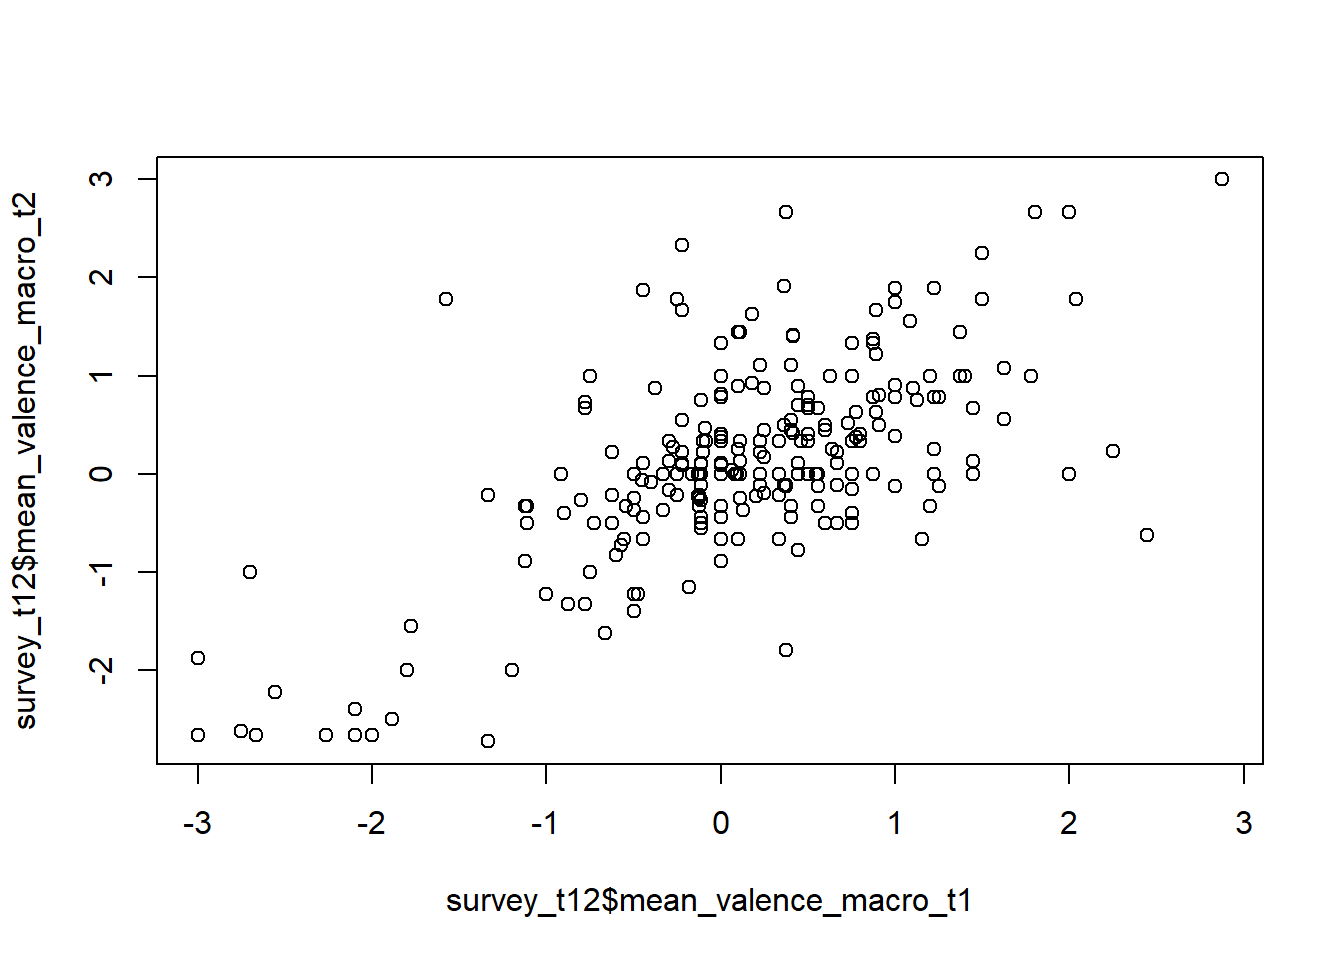
\includegraphics{02_analysis_files/figure-latex/unnamed-chunk-25-1} \end{center}

\emph{we will perform linear regressions with the indicated mental model
network indicators as DV and dummy coded group differences as IV
(no/yes-intention, high/low climate concern, left/right political
orientation). In the case of the latter two, we may also use a
continuous DV to assess correlation with network properties. We will
control for socio-demographic variables (gender, age, education).}

With mean valence macro

\textbf{Intended vote}

Supported

~

mean\_valence\_macro\_t1

Predictors

Estimates

CI

p

(Intercept)

-0.62

-1.04~--~-0.21

0.003

intendedVote

0.75

0.51~--~0.98

\textless0.001

age

0.01

-0.00~--~0.01

0.161

gender {[}weiblich{]}

0.05

-0.17~--~0.27

0.659

education {[}linear{]}

-0.22

-0.41~--~-0.03

0.024

education {[}quadratic{]}

0.08

-0.11~--~0.28

0.411

Observations

254

R2 / R2 adjusted

0.154 / 0.137

~

mean\_valence\_macro\_t1

Predictors

Estimates

CI

p

(Intercept)

-1.32

-1.77~--~-0.87

\textless0.001

ratingLaw

0.22

0.17~--~0.27

\textless0.001

age

0.01

-0.00~--~0.01

0.076

gender {[}weiblich{]}

0.04

-0.17~--~0.24

0.729

education {[}linear{]}

-0.27

-0.45~--~-0.09

0.004

education {[}quadratic{]}

0.07

-0.11~--~0.25

0.436

Observations

254

R2 / R2 adjusted

0.257 / 0.243

\textbf{Climate change concern}

Supported

~

mean\_valence\_macro\_t1

Predictors

Estimates

CI

p

(Intercept)

-1.30

-1.82~--~-0.77

\textless0.001

climate concern

0.29

0.20~--~0.37

\textless0.001

age

0.00

-0.01~--~0.01

0.617

gender {[}weiblich{]}

0.04

-0.18~--~0.26

0.732

education {[}linear{]}

-0.22

-0.41~--~-0.03

0.022

education {[}quadratic{]}

0.07

-0.12~--~0.27

0.461

Observations

254

R2 / R2 adjusted

0.172 / 0.155

\textbf{Political orientation}

Supported (but when excluding climate concern and vote no longer)

~

mean\_valence\_macro\_t1

Predictors

Estimates

CI

p

(Intercept)

0.56

0.08~--~1.04

0.023

politicalOrientation

-0.10

-0.16~--~-0.04

0.001

age

0.00

-0.01~--~0.01

0.608

gender {[}weiblich{]}

0.03

-0.21~--~0.26

0.831

education {[}linear{]}

-0.22

-0.42~--~-0.02

0.033

education {[}quadratic{]}

0.14

-0.07~--~0.35

0.180

Observations

254

R2 / R2 adjusted

0.059 / 0.040

\textbf{All three}

~

mean\_valence\_macro\_t1

Predictors

Estimates

CI

p

(Intercept)

-1.23

-1.94~--~-0.52

0.001

politicalOrientation

-0.01

-0.07~--~0.06

0.819

intendedVote

0.44

0.16~--~0.72

0.002

climate concern

0.20

0.09~--~0.30

\textless0.001

age

0.00

-0.00~--~0.01

0.259

gender {[}weiblich{]}

0.04

-0.18~--~0.25

0.742

education {[}linear{]}

-0.23

-0.42~--~-0.05

0.015

education {[}quadratic{]}

0.07

-0.12~--~0.26

0.496

Observations

254

R2 / R2 adjusted

0.206 / 0.183

~

mean\_valence\_macro\_t1

Predictors

Estimates

CI

p

(Intercept)

-1.61

-2.31~--~-0.91

\textless0.001

politicalOrientation

0.01

-0.05~--~0.07

0.674

ratingLaw

0.19

0.12~--~0.26

\textless0.001

climate concern

0.09

-0.02~--~0.20

0.099

age

0.01

-0.00~--~0.01

0.112

gender {[}weiblich{]}

0.04

-0.17~--~0.25

0.723

education {[}linear{]}

-0.26

-0.44~--~-0.08

0.004

education {[}quadratic{]}

0.06

-0.12~--~0.24

0.509

Observations

254

R2 / R2 adjusted

0.266 / 0.245

\hypertarget{wave-2}{%
\paragraph{wave 2}\label{wave-2}}

No major differences to wave 1 results

\textbf{Intended vote \& rating of law}

Supported

~

mean\_valence\_macro\_t2

Predictors

Estimates

CI

p

(Intercept)

-0.80

-1.22~--~-0.37

\textless0.001

intendedVote

0.95

0.71~--~1.19

\textless0.001

age

0.01

-0.00~--~0.01

0.123

gender {[}weiblich{]}

0.12

-0.11~--~0.35

0.324

education {[}linear{]}

-0.13

-0.32~--~0.07

0.207

education {[}quadratic{]}

0.12

-0.08~--~0.32

0.241

Observations

254

R2 / R2 adjusted

0.214 / 0.198

~

mean\_valence\_macro\_t2

Predictors

Estimates

CI

p

(Intercept)

-1.59

-2.03~--~-1.16

\textless0.001

ratingLaw

0.26

0.22~--~0.31

\textless0.001

age

0.01

-0.00~--~0.01

0.066

gender {[}weiblich{]}

0.11

-0.10~--~0.32

0.308

education {[}linear{]}

-0.12

-0.30~--~0.06

0.197

education {[}quadratic{]}

0.10

-0.09~--~0.28

0.308

Observations

254

R2 / R2 adjusted

0.352 / 0.339

\textbf{Climate change concern}

~

mean\_valence\_macro\_t2

Predictors

Estimates

CI

p

(Intercept)

-1.49

-2.06~--~-0.93

\textless0.001

climate concern

0.32

0.23~--~0.41

\textless0.001

age

0.00

-0.01~--~0.01

0.573

gender {[}weiblich{]}

0.07

-0.16~--~0.31

0.547

education {[}linear{]}

-0.14

-0.34~--~0.06

0.169

education {[}quadratic{]}

0.11

-0.09~--~0.32

0.276

Observations

254

R2 / R2 adjusted

0.183 / 0.167

\textbf{Political orientation}

~

mean\_valence\_macro\_t2

Predictors

Estimates

CI

p

(Intercept)

0.71

0.20~--~1.22

0.007

politicalOrientation

-0.14

-0.20~--~-0.07

\textless0.001

age

0.00

-0.01~--~0.01

0.528

gender {[}weiblich{]}

0.05

-0.20~--~0.30

0.697

education {[}linear{]}

-0.15

-0.36~--~0.07

0.182

education {[}quadratic{]}

0.20

-0.02~--~0.41

0.080

Observations

254

R2 / R2 adjusted

0.079 / 0.060

\hypertarget{specification-under-the-curve-analysis-emotional-properties}{%
\paragraph{specification under the curve analysis emotional
properties}\label{specification-under-the-curve-analysis-emotional-properties}}

\begin{center}\includegraphics{02_analysis_files/figure-latex/unnamed-chunk-37-1} \end{center}

\begin{verbatim}
## Scale for fill is already present.
## Adding another scale for fill, which will replace the existing scale.
\end{verbatim}

\begin{center}\includegraphics{02_analysis_files/figure-latex/unnamed-chunk-37-2} \end{center}

Standardized

\begin{center}\includegraphics{02_analysis_files/figure-latex/unnamed-chunk-38-1} \end{center}

\begin{verbatim}
## Scale for fill is already present.
## Adding another scale for fill, which will replace the existing scale.
\end{verbatim}

\begin{center}\includegraphics{02_analysis_files/figure-latex/unnamed-chunk-38-2} \end{center}

Standardized \textbf{climate concern }

\begin{center}\includegraphics{02_analysis_files/figure-latex/unnamed-chunk-39-1} \end{center}

\begin{verbatim}
FALSE Scale for fill is already present.
FALSE Adding another scale for fill, which will replace the existing scale.
\end{verbatim}

\begin{center}\includegraphics{02_analysis_files/figure-latex/unnamed-chunk-39-2} \end{center}

\hypertarget{hypothesis-2}{%
\subsubsection{Hypothesis 2}\label{hypothesis-2}}

\hypertarget{latent-properties}{%
\subparagraph{Latent properties}\label{latent-properties}}

\emph{We will explore differences in latent properties of mental models
of {[}those intending to vote yes versus no on the upcoming climate
protection law{]}. }

Rating of law and climate change concern\\
\textbf{Density indicator}\\
Both are close to significance but not quite

~

density\_macro\_t1

Predictors

Estimates

CI

p

(Intercept)

0.27

0.26~--~0.29

\textless0.001

climate concern

0.01

-0.00~--~0.02

0.074

age

0.01

0.00~--~0.02

0.028

gender {[}weiblich{]}

-0.01

-0.03~--~0.01

0.360

education {[}linear{]}

0.03

0.01~--~0.05

0.005

education {[}quadratic{]}

0.00

-0.02~--~0.02

0.726

Observations

254

R2 / R2 adjusted

0.071 / 0.053

~

density\_macro\_t1

Predictors

Estimates

CI

p

(Intercept)

0.27

0.26~--~0.29

\textless0.001

ratingLaw

0.01

-0.00~--~0.02

0.093

age

0.01

0.00~--~0.02

0.017

gender {[}weiblich{]}

-0.01

-0.03~--~0.01

0.366

education {[}linear{]}

0.03

0.01~--~0.05

0.006

education {[}quadratic{]}

0.00

-0.02~--~0.02

0.702

Observations

254

R2 / R2 adjusted

0.070 / 0.051

Rating of law and climate change concern

\textbf{Number of nodes indicator}\\
Climate concern close \textasciitilde{} approaching significance

~

num\_nodes\_macro\_t1

Predictors

Estimates

CI

p

(Intercept)

9.69

9.34~--~10.05

\textless0.001

climate concern

-0.20

-0.47~--~0.07

0.150

age

-0.31

-0.59~--~-0.04

0.024

gender {[}weiblich{]}

-0.06

-0.61~--~0.49

0.828

education {[}linear{]}

-0.40

-0.87~--~0.07

0.097

education {[}quadratic{]}

0.13

-0.35~--~0.61

0.602

Observations

254

R2 / R2 adjusted

0.039 / 0.019

~

num\_nodes\_macro\_t1

Predictors

Estimates

CI

p

(Intercept)

9.70

9.34~--~10.06

\textless0.001

ratingLaw

-0.02

-0.30~--~0.25

0.880

age

-0.31

-0.59~--~-0.03

0.028

gender {[}weiblich{]}

-0.07

-0.62~--~0.48

0.798

education {[}linear{]}

-0.41

-0.89~--~0.06

0.088

education {[}quadratic{]}

0.10

-0.38~--~0.59

0.671

Observations

254

R2 / R2 adjusted

0.031 / 0.011

\hypertarget{specification-under-the-curve-analysis-latent-properties}{%
\paragraph{specification under the curve analysis latent
properties}\label{specification-under-the-curve-analysis-latent-properties}}

Rating of law

\begin{center}\includegraphics{02_analysis_files/figure-latex/unnamed-chunk-44-1} \end{center}

\begin{verbatim}
FALSE Scale for fill is already present.
FALSE Adding another scale for fill, which will replace the existing scale.
\end{verbatim}

\begin{center}\includegraphics{02_analysis_files/figure-latex/unnamed-chunk-44-2} \end{center}

Standardized rating of law

\begin{center}\includegraphics{02_analysis_files/figure-latex/unnamed-chunk-45-1} \end{center}

\begin{verbatim}
FALSE Scale for fill is already present.
FALSE Adding another scale for fill, which will replace the existing scale.
\end{verbatim}

\begin{center}\includegraphics{02_analysis_files/figure-latex/unnamed-chunk-45-2} \end{center}

With climate change concern as predictor

\begin{center}\includegraphics{02_analysis_files/figure-latex/unnamed-chunk-46-1} \end{center}

\begin{verbatim}
## Scale for fill is already present.
## Adding another scale for fill, which will replace the existing scale.
\end{verbatim}

\begin{center}\includegraphics{02_analysis_files/figure-latex/unnamed-chunk-46-2} \end{center}

\hypertarget{hypothesis-3-content}{%
\subsubsection{Hypothesis 3 content}\label{hypothesis-3-content}}

\hypertarget{hypothesis-4}{%
\subsubsection{Hypothesis 4}\label{hypothesis-4}}

\emph{We expect that evaluation of the law will be positively correlated
with the emotional properties of mental models. Such that a more
positive evaluation of the law will be associated with more positive
valence.}

Supported\\

~

mean\_valence\_macro\_t1

Predictors

Estimates

CI

p

(Intercept)

0.01

-0.13~--~0.16

0.877

ratingLaw

0.50

0.39~--~0.61

\textless0.001

age

0.10

-0.01~--~0.21

0.076

gender {[}weiblich{]}

0.04

-0.18~--~0.26

0.729

education {[}linear{]}

-0.28

-0.48~--~-0.09

0.004

education {[}quadratic{]}

0.08

-0.12~--~0.27

0.436

Observations

254

R2 / R2 adjusted

0.257 / 0.243

\begin{center}\includegraphics{02_analysis_files/figure-latex/unnamed-chunk-47-1} \end{center}

\begin{verbatim}
FALSE `geom_smooth()` using method = 'loess' and formula = 'y ~ x'
\end{verbatim}

\begin{center}\includegraphics{02_analysis_files/figure-latex/unnamed-chunk-47-2} \end{center}

\hypertarget{longitudinal}{%
\subsection{Longitudinal}\label{longitudinal}}

\hypertarget{hypothesis-5}{%
\subsubsection{Hypothesis 5}\label{hypothesis-5}}

\emph{We expect to find temporal differences in latent properties of
mental models from wave 2 to wave 1. Such that the complexity of mental
models will increase from wave 1 to wave 2. }

Not supported

\begin{center}\includegraphics{02_analysis_files/figure-latex/unnamed-chunk-49-1} \end{center}

\begin{center}\includegraphics{02_analysis_files/figure-latex/unnamed-chunk-49-2} \end{center}

~

num\_nodes\_macro

Predictors

Estimates

CI

p

(Intercept)

8.80

4.82~--~12.78

\textless0.001

wave {[}t2{]}

0.07

-0.24~--~0.38

0.646

media engagement rel

0.02

-0.23~--~0.27

0.862

ratingLaw

0.08

-0.02~--~0.19

0.123

age

-0.02

-0.04~--~-0.00

0.018

gender {[}Keine Angabe{]}

-0.36

-5.85~--~5.12

0.896

gender {[}männlich{]}

1.43

-2.45~--~5.30

0.469

gender {[}weiblich{]}

1.14

-2.74~--~5.02

0.565

education {[}linear{]}

-0.42

-0.85~--~0.01

0.057

education {[}quadratic{]}

0.04

-0.39~--~0.48

0.847

Random Effects

σ2

3.18

τ00 participantID

2.22

ICC

0.41

N participantID

256

Observations

512

Marginal R2 / Conditional R2

0.038 / 0.433

~

density\_macro

Predictors

Estimates

CI

p

(Intercept)

0.25

0.08~--~0.42

0.005

wave {[}t2{]}

0.01

-0.01~--~0.02

0.210

media engagement rel

0.01

-0.00~--~0.02

0.165

ratingLaw

0.00

-0.00~--~0.01

0.456

age

0.00

0.00~--~0.00

0.006

gender {[}Keine Angabe{]}

-0.04

-0.27~--~0.20

0.764

gender {[}männlich{]}

-0.03

-0.20~--~0.13

0.691

gender {[}weiblich{]}

-0.03

-0.19~--~0.14

0.741

education {[}linear{]}

0.02

0.00~--~0.04

0.030

education {[}quadratic{]}

-0.00

-0.02~--~0.02

0.739

Random Effects

σ2

0.01

τ00 participantID

0.00

ICC

0.37

N participantID

256

Observations

512

Marginal R2 / Conditional R2

0.042 / 0.395

~

density\_macro

Predictors

Estimates

CI

p

(Intercept)

0.25

0.09~--~0.42

0.003

wave {[}t2{]}

0.01

-0.00~--~0.02

0.204

media engagement rel

0.01

-0.00~--~0.02

0.176

climate concern rel

0.01

-0.00~--~0.02

0.231

age

0.00

0.00~--~0.00

0.007

gender {[}Keine Angabe{]}

-0.03

-0.26~--~0.21

0.833

gender {[}männlich{]}

-0.03

-0.20~--~0.14

0.719

gender {[}weiblich{]}

-0.03

-0.19~--~0.14

0.766

education {[}linear{]}

0.02

0.00~--~0.04

0.031

education {[}quadratic{]}

-0.00

-0.02~--~0.02

0.706

Random Effects

σ2

0.01

τ00 participantID

0.00

ICC

0.37

N participantID

256

Observations

512

Marginal R2 / Conditional R2

0.045 / 0.396

\emph{H5a: This effect may be moderated by engagement with the topic.
Such that those that spend more time researching or discussing the topic
show an even higher increase in complexity of mental models. }

Not supported

~

density\_macro

Predictors

Estimates

CI

p

(Intercept)

0.25

0.09~--~0.42

0.003

wave {[}t2{]}

0.01

-0.00~--~0.02

0.204

media engagement rel

0.01

-0.00~--~0.02

0.143

climate concern rel

0.01

-0.00~--~0.02

0.231

age

0.00

0.00~--~0.00

0.007

gender {[}Keine Angabe{]}

-0.03

-0.26~--~0.21

0.833

gender {[}männlich{]}

-0.03

-0.20~--~0.14

0.719

gender {[}weiblich{]}

-0.03

-0.19~--~0.14

0.766

education {[}linear{]}

0.02

0.00~--~0.04

0.031

education {[}quadratic{]}

-0.00

-0.02~--~0.02

0.706

wave {[}t2{]} × mediaengagement rel

-0.00

-0.02~--~0.01

0.540

Random Effects

σ2

0.01

τ00 participantID

0.00

ICC

0.37

N participantID

256

Observations

512

Marginal R2 / Conditional R2

0.045 / 0.396

\hypertarget{specification-curve-analysis-longitdunal}{%
\paragraph{Specification curve analysis
longitdunal}\label{specification-curve-analysis-longitdunal}}

\begin{verbatim}
FALSE Scale for fill is already present.
FALSE Adding another scale for fill, which will replace the existing scale.
\end{verbatim}

\begin{center}\includegraphics{02_analysis_files/figure-latex/unnamed-chunk-52-1} \end{center}

\hypertarget{hypothesis-6}{%
\subsubsection{Hypothesis 6}\label{hypothesis-6}}

\emph{H6: We expect temporal changes such that emotional properties will
become more extreme over time (higher or lower valence). We expect an
interaction effect as a function of {[}intended vote{]}. Such that
{[}yes (no) intention-voters{]} will show an increase (decrease) in
positive valence. }

Not supported (p=.145)

~

mean\_valence\_macro

Predictors

Estimates

CI

p

(Intercept)

0.11

-1.45~--~1.67

0.886

wave {[}t2{]}

-0.09

-0.27~--~0.09

0.321

intendedVote

0.27

0.05~--~0.50

0.018

climate concern rel

0.29

0.18~--~0.40

\textless0.001

media engagement rel

0.03

-0.06~--~0.13

0.500

age

0.00

-0.00~--~0.01

0.246

gender {[}Keine Angabe{]}

-0.40

-2.59~--~1.79

0.722

gender {[}männlich{]}

-0.36

-1.90~--~1.18

0.644

gender {[}weiblich{]}

-0.30

-1.84~--~1.24

0.704

education {[}linear{]}

-0.20

-0.37~--~-0.02

0.026

education {[}quadratic{]}

0.09

-0.08~--~0.26

0.297

wave {[}t2{]} × intendedVote

0.16

-0.07~--~0.38

0.172

Random Effects

σ2

0.33

τ00 participantID

0.44

ICC

0.57

N participantID

256

Observations

512

Marginal R2 / Conditional R2

0.198 / 0.658

\textbf{Exploratory: Media engagement by intended vote}\\
To be discussed: The media engagment item was phrased as: How did you
inform yourself about the climate law and the vote \textbf{in the past
month} this may in itself be a temproal effect?

Not significant relationship, but approaches significance (p =.055)

~

mean\_valence\_macro

Predictors

Estimates

CI

p

(Intercept)

0.08

-1.47~--~1.64

0.916

wave {[}t2{]}

0.02

-0.08~--~0.12

0.737

media engagement rel

-0.13

-0.30~--~0.05

0.149

intendedVote {[}yes{]}

0.35

0.16~--~0.55

\textless0.001

climate concern rel

0.31

0.19~--~0.42

\textless0.001

age

0.00

-0.00~--~0.01

0.214

gender {[}Keine Angabe{]}

-0.29

-2.48~--~1.90

0.794

gender {[}männlich{]}

-0.40

-1.94~--~1.14

0.611

gender {[}weiblich{]}

-0.36

-1.90~--~1.18

0.646

education {[}linear{]}

-0.20

-0.37~--~-0.03

0.023

education {[}quadratic{]}

0.07

-0.10~--~0.24

0.434

wave {[}t2{]} × mediaengagement rel

0.06

-0.04~--~0.16

0.237

media engagement rel ×intendedVote {[}yes{]}

0.18

-0.00~--~0.36

0.054

Random Effects

σ2

0.32

τ00 participantID

0.43

ICC

0.57

N participantID

256

Observations

512

Marginal R2 / Conditional R2

0.203 / 0.659

\begin{center}\includegraphics{02_analysis_files/figure-latex/unnamed-chunk-54-1} \end{center}

\hypertarget{hypothesis-7}{%
\paragraph{Hypothesis 7}\label{hypothesis-7}}

Number of ambivalent concepts is 0 for both waves\ldots{}

\begin{verbatim}
##    
##      t1  t2 wave2_control
##   0 113 146            41
##   1  77  61            20
##   2  45  29             5
##   3   9  12             2
##   4   6   2             0
##   5   3   4             2
##   6   0   1             0
##   7   0   1             1
##   8   3   0             1
\end{verbatim}

\begin{verbatim}
## 
##  Paired t-test
## 
## data:  survey_t1_CAM$num_nodes_ambi_macro_t1 and survey_t2_CAM$num_nodes_ambi_macro_t2
## t = 2.5124, df = 253, p-value = 0.01261
## alternative hypothesis: true mean difference is not equal to 0
## 95 percent confidence interval:
##  0.05020592 0.41436101
## sample estimates:
## mean difference 
##       0.2322835
\end{verbatim}

\begin{verbatim}
## 
##  Wilcoxon signed rank test with continuity correction
## 
## data:  survey_t1_CAM$num_nodes_ambi_macro_t1 and survey_t2_CAM$num_nodes_ambi_macro_t2
## V = 5597.5, p-value = 0.008163
## alternative hypothesis: true location shift is not equal to 0
\end{verbatim}

\begin{center}\includegraphics{02_analysis_files/figure-latex/unnamed-chunk-56-1} \end{center}

\hypertarget{exploratory-analysis}{%
\subsubsection{exploratory analysis}\label{exploratory-analysis}}

\hypertarget{mixed}{%
\section{Mixed}\label{mixed}}

\hypertarget{references}{%
\section{References}\label{references}}

\end{document}
